\documentclass[twocolumn]{article}

\usepackage{graphicx}
\usepackage{amsmath}
\usepackage{amsfonts}
\usepackage{floatpag}
\usepackage{caption}


\title{3D Environment Generation Using Conditional Adversarial Networks}

\author{Tim Whitaker \\ Colorado State University}

\begin{document}

	\maketitle
	
	\section{Abstract}
	
	We introduce a method and application for generating 3D environments using conditional generative adversarial networks. The outputs from our networks are able to be imported into popular three dimensional modeling software like Unreal, Unity and Blender. We've created a simple web based interface to allow a user to control the output of the generated environment by painting with predefined brushes that represent terrain varieties: mountains, hills, terraces, plains, and rivers.
	
	\section{Introduction}

	This project explores the usage of conditional generative adversarial networks to synthesize 3 dimensional environments.
	
	The motivations for this project are to make it easier for game, world or environment designers to create realistic environments procedurally while giving the designer more control over the results.
	
	We aim to create a simple and easy to use GUI interface for a user to paint a 2 dimensional semantically significant image map. We then pass the user created image map through a generative adversarial network trained on elevation data gathered from the Earth in order to generate a realistic terrain heightmap that approximately represents the user defined map. The resulting heightmap produced from the neural network can then be uploaded into any of the popular 3 dimensional rendering softwares including Unity, Unreal, Blender or World Machine.
	
	This approach offers a promising avenue to co-creative design. Humans working together with machine learning programs could allow for more creative results with reduced cost and effort for the designer. The flexibility of being able to tweak and tune the training set also allows for the possibility of adapting this approach to content of many different kinds, not just 3d environments.
	
	\section{Background}
			
	\subsection{Procedural Content Generation}
	
	Procedural content generation is an algorithmic and stochastic process used in art, games, music and film. As a paradigm for content generation, it is used to increase replayability, variability, flexibility and reduce production cost, effort and storage space \cite{summerville2017procedural}. These algorithms are crafted by hand and they require a lot of tuning by a developer to ensure that the random perturbations result in usable content.
	
	Procedral content generation has been used in production applications since 1980 with the dungeon crawler Rogue demonstrating its effectiveness. \cite{wiki:procedural} Procedural generation has been a staple in gaming since and today it continues to be featured in some of the top games.
	
	The addition of machine learning to procedural generation is a new topic in research. Most projects are using 2 dimensional platformers, but real time strategy and 3 dimensional environments are also being explored. This field of research has its own challenges, particularly the comparability of results, but efforts are beng made to improve benchmarks and datasets \cite{summerville2017procedural}.

	\subsection{Generative Adversarial Networks}
	
	Neural networks allow for a powerful model of learning patterns from complex datasets. Generative adversarial networks work by synthesizing novel data according to patterns it learns in the training set. They work by training two neural networks in competition with each other, a generator and a discriminator. The generator network generates new data instances and the discriminator classifies the results of the generator according to how authentic the generated images are given some training distribution. These two networks train in tandem, and over time, the generator gets good at producing novel images that look like they belong to the training set.
		
	We are evaluate two implementations of a specialized form of generative adversarial networks designed to perform conditional image to image translation. The two models we are using are called Pix2Pix and CycleGAN.
	
	The objective function of a standard conditional generative adversarial network can be expressed as:
	
	\begin{align*}
		\mathcal{L}_{cGAN}(G, D) &= \mathbb{E}_{x,y}[log(D(x, y))] \\
		&+ \mathbb{E}_{x,z}[log(1 - D(x, G(x, z))]
	\end{align*}
	
	Where $G$ is the generator network that is attempting to minimize this objective and D is the discriminator network that tries to maximize it.

	Pix2Pix and CycleGAN both make modifications to this objective function and below we go into those changes.	
	
	\subsubsection{Pix2Pix}	
	
	Pix2Pix introduces a a generalized approach to image to image translation problems.  Their model learns not only a mapping between input and output images, but it also learns a loss function between the two image datasets. This allows this model to be used for a variety of image tasks that would originally need very different model and loss configurations \cite{isola2016imagetoimage}.
	
	Pix2Pix found it beneficial to add a traditional loss term as well, namely L1 distance. The discriminators job is the same as a traditional GAN, but the generator now is tasked with fooling the discriminator as well as producing results near the ground truth output.
	
	$$
		\mathcal{L}_{L1}(G) = \mathbb{E}_{x,y,z}[|| y - G(x, z) ||_1]		
	$$

	The addition of that loss term can be tuned with a parameter  $\lambda$. This combined objective function is used for training Pix2Pix.
	
	$$	
		G^* = arg \mathop{min}_G \mathop{max}_D \mathcal{L}_{cGAN}(G, D) + \lambda \mathcal{L}_{L1}(G)
	$$
	
	\subsubsection{CycleGAN}
	
	CycleGAN introduces cycle consistency loss to conditional generative adversarial networks. It works by measuring the loss of a mapping from one distribution to another and then back to the original distribution again. This approach allows for good generalization and the advantage of not needing specifically paired images in the training distributions. This can save a lot of time in building large datasets, but it can lose out on the specificity offered by Pix2Pix \cite{zhu2017unpaired}.
	
	Where pix2pix trains one GAN (one generator and one discriminator), CycleGAN trains two, (Generator A and B and Discriminator A and B). Learning the mapping between the two GANs is the trick to getting unpaired image translation to work. CycleGAN introduces a cycle consistency loss. The idea is that for each image in the $x$ domain, the image translation cycle should be able to bring the $x$ back to the original image, $x \rightarrow G(x) \rightarrow F(G(x)) \approx x$.
	
	\begin{align*}
		\mathcal{L}_{cyc}(G, F) =\ & \mathbb{E}_{x,y}[||F(G(x)) - x||_1]\ + \\
		& \mathbb{E}_{x,z}[||G(F(y)) - y||_1]
	\end{align*}
	
	This cycle consistency loss is then combined with the standard GAN loss for each GAN:
	
	\begin{align*}
		\mathcal{L}(G, F, D_X, D_Y) &=\ \mathcal{L}_{GAN}(G, D_Y, X, Y) \\
		&+\ \mathcal{L}_{GAN}(F, D_X, Y, X) \\
		&+\ \lambda \mathcal{L}_cyc (G, F)  
	\end{align*}
	
	The generators then seek to minimize this objective while the discriminators try to maximize it.
	
	\begin{align*}
		G^*, F^* = arg \mathop{min}_{G,F} \mathop{max}_{D_x, D_y} \mathcal{L}(G, F, D_x, D_y)
	\end{align*}

	\subsection{Related Work}
	
	\subsubsection{Nvidia's GauGAN}
	
	GauGAN was the inspiration behind the semantic user map. This research demonstrated an application that took a 2 dimensional semantic image drawn by a user, and translated it into a photorealistic image. This project also used Pix2Pix as a base for their network architecture, but they also introduce a novel normalization layer called spatially-adaptive normalization. The idea is that normal layer normalization tends to wash out semantic meaning from an image. By considering the spatial properties, you can keep the semantic information in tact while still performing normalization. \cite{park2019semantic}	. Nvidia hosts an excellent demo of the project at http://nvidia-research-mingyuliu.com/gaugan.
	
	
	\subsubsection{A Step Toward Procedural Terrain Generation with GANs}
	
	This paper had a very similar idea to this project. They use a standard generative adversarial network to synthesize terrain heightmaps with a model trained on Earth data. They use NASA's visible earth project for their training image data at a resolution of 1km per pixel. This project appears to be quite introductory and they lay out a good overview of how a standard GAN could be implemented to generate environments. We expand on their work by introducing the conditional GAN and integrating co-creative design by including a translation from a user defined segmentation map. \cite{beckham2017step}
		
	\section{Methodology}
		
	\subsection{User Interface Application}
	
	The user interface is a web based javascript application that allows a user to paint a semantically significant image using predefined brushes. We include tools to change the brush size and export or clear the image. The canvas size is 512 x 512 pixels, and these images are resized automatically when passed to our neural network.

	\begin{figure}[h!]
	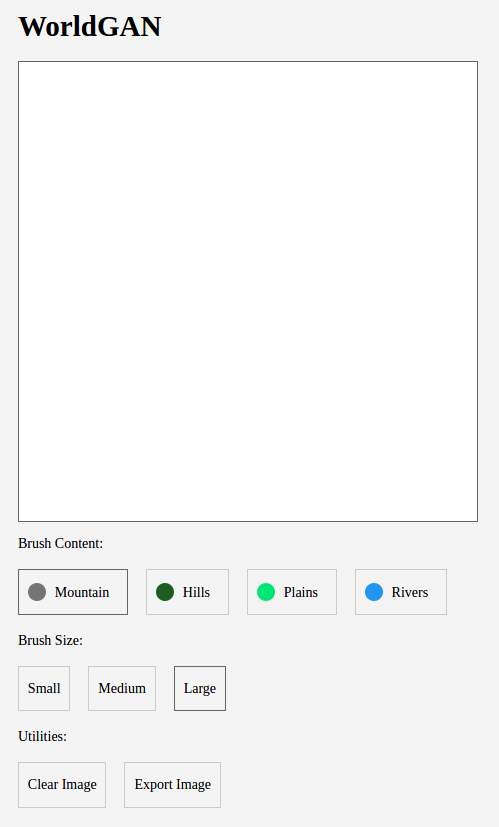
\includegraphics[width=1\columnwidth]{ui.png} 
	\caption{The user interace application}
	\end{figure}
	
	The backend is powered by a Flask API. We set up an endpoint to be able to evaluate a drawn image on our trained models. In order to pass the usermap and generated heightmap back and forth between the client and the server, we use base 64 encoding and decoding on the image. This way we can save the images to the file system and have a local process run the neural network and return the generated heightmap. This direct access to the file system has security concerns, so it's only recommended to run the app locally.
	
	\subsection{The Dataset}
	
	Generative adversarial networks need a good amount of training data to output good results and a key objective of this project is to generate realistic results. This leads to an interesting challenge of putting together a realistic yet sizable dataset. In order to achieve this, we use terrain data of the Earth as opposed to fictional or manufactured terrain data. In the next two sections we go into the methodology behind building the dataset.

	\subsubsection{Training Data}
	
	We use an interactive open source map tool that visualizes elevation data gathered from Mapzen's global elevation service \cite{richardson2016mapzen}. The data for the map tool is aggregated from 3 sources, USGS, NASA, and NGA. The map is a greyscale map, where the brightness of the pixel corresponds to the relative elevation.
	
	We then built a program that controls a headless browser using an open source library developed by Google called Puppeteer. This script loads a random coordinate, checks if the coordinate is over land and if so, then we save an image of the elevation data at that coordinate. We resize the saved image to be 512 x 512 pixels.
	
	We then manually build the usermap training set using our user interface application. For each image in the heightmap training set, we paint a usermap to represent that heightmap, using the semantically significant brushes that most closely match the terrain (mountains, hills, plains, rivers, and terraces). This process is a subjective one and all usermaps were painted by myself. This does bias the model to produce images according to how I read the heightmaps.

	After this process we are left with 258 paired usermaps and heightmaps. We group all of these together into a batch to be trained on.

	Creating the usermaps by hand is quite time consuming, and I wanted to experiment with models trained on a large dataset. We accomplish this by augmenting our first batch with simple transformations in order to artificially increase the number of images we can train on. Image augmentations are a well researched and effective appoach to improving neural network performance \cite{perez2017effectiveness}.
	
	We performed 5 operations on each usermap and heightmap. We mirror horizontally, flip vertically, rotate 90 derees, rotate 180 degrees, and rotate 270 degrees.	All of the resulting images are gathered into a second batch and we end up with 1548 paired images (a 5x increase).
	
	Before training the networks, we need to perform one more preprocessing step. Pix2Pix requires paired images to be combined into a single side by side image. We stack each pair of usermap and heightmap and save these images into separate batches spcifically for Pix2Pix. Each resulting image is 1024 x 512 pixels. CycleGAN does not need this preprocessing step and can be trained on images in different directories.
			
	\subsubsection{Test Data}
	
	The test data is a collection of 10 usermaps I drew that are designed to be representative of a variety of environments a user might draw. These 10 environments include mountainous regions, hilly regions, flat regions and combined regions.
	
	\subsection{Training The Models}
	
	We trained a total of 4 models. Pix2Pix and CycleGAN on both the original and augmented batch of training data. The training was performed on my desktop GPU enabled PC. The operating system is Ubuntu 18.04. We train on a Nvidia GTX 1080ti GPU with 11 GB of memory, an Intel i7 8700k processor, a 500GB solid state hard drive, and 32 GB of RAM.
	
	Both models are built on top of the PyTorch framework \cite{paszke2019pytorch} and are trained for 200 epochs. We use the default hyperparameters of 0.0002 for the learning rate and ADAM for the optimizer. We use the open source repo implemented by Jun-Yan Zhu, who published the research on both models \cite{junyanzhu2017github}. Both models are 15 layers deep and contain multiple convolutional layers and residual blocks \cite{isola2016imagetoimage} \cite{zhu2017unpaired}.
	
	\subsubsection{Pix2Pix}
		Our pix2pix model contains a total of 57.183 million parameters. The generator network contains 54.414 million parameters and the discriminator contains 2.769 million parameters. The original batch of data took approximately 45 minutes to train. The augmented batch took approximately 4 hours to train.
	
	\subsubsection{CycleGAN}
		Our cyclegan model contained a total of 28.286 million parameters. Generator A and Generator B each contain 11.378 million parameters. Discriminator A and Discriminator B each contain 2.765 million parameters. The original batch of data took approximately 4 hours to train. The augmented batch took approximately 24 hours to train.

	\subsection{Visualizations Using 3D Software}
	
	The resulting heightmaps can be imported into popular 3d modeling software including Unity, Unreal, Blender, and World Machine. For the purposes of visualizing these results, and because of the limited support for Linux, we visualize results using a demo application called Fractscape. Fractscape includes elevation based texture mapping which happens to work very well for visualizing our terrain elevation data. Unity, Unreal, Blender and World Machine all have different workflows for painting textures, so using the generality of fractscape works best for our visualizations \cite{starscenesoftware2006}.

	\section{Results}
	
	Subjective results of networks show that Pix2Pix performs much better than CycleGAN. For the specfic task of segmented image translation, paired training data allows the network to learn the meaning of the segmentations much better. Cyclegan had issues of keeping the semantic meaning in tact. Even though it does appear to generate some of the patterns correctly, it's often mapped to the wrong brush or user defined section.
	
	Both models trained on the augmented batch produce higher fidelity images. Both Pix2Pix models produce usable and realistic terrain.
	
	We also find that the model does not perform very well on usermaps with rivers. We found that rivers tend to produce noisy results and sometimes the rivers aren't defined enough to be noticeable in the results. I think this can be solved with more training data including rivers. Due to the nature of how the training data was gathered, it's likely that we didn't get enough examples, and due to the subjective nature of myself reading the earth data and drawing the usermaps myself, I could have read them wrong and not painted them as detailed as they needed to be.

	Terraces also had a lack of training data. Due to the specificity of their appearance, they were able to produce better results than rivers. The models will likely struggle on terraces with odd shapes.

	Mountains, hills, and plains all performed very well. There was plenty of samples in the training for these features and the areas for each tend to be large. This allowed the networks to do a great job of modeling these terrain features.

	\subsection{User Preference Survey}
	
	We also created a small user survey to measure user preference between the 4 trained models. The survey was conducted through google forms and sent to the students in CSCI 567 (3D User Interfaces) through the piazza message board. I took a sample of 5 user maps, and for each one, I produced the ouput for each model and listed those as multiple choice answers.
	
	We recieved 11 responses. For all 5 samples, users preferred the output of Pix2Pix over the output of CycleGAN. When looking at the results of the original training batch to the augmented training batch, users preferred the ouput of the original batch for 4 samples and the augmented batch for one of the samples.

	\begin{table*}[h]
		\begin{tabular}{c|c|c|c|c}
			Sample Number & Original Pix2Pix & Augmented Pix2Pix & Original CycleGAN & Augmented CycleGAN \\
			\hline
			1 & 6 & 3 & 1 & 1 \\
			2 & 8 & 1 & 1 & 1 \\
			3 & 3 & 6 & 2 & 0 \\
			4 & 5 & 4 & 1 & 1 \\
			5 & 7 & 3 & 1 & 0
		\end{tabular}
		
	\caption{Survey Results}
	\end{table*}	
	
	\begin{table*}[t]
	\thisfloatpagestyle{empty}
	\vspace{-2cm}
		\begin{tabular}{c|c|c|c|c}
 			Test Image & Original Pix2Pix & Augmented Pix2Pix & Original CycleGAN & Augmented CycleGAN \\
 			\hline
 				
\includegraphics[trim=0 0 0 -20, width=0.25\columnwidth]{00.png} & 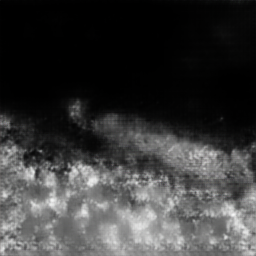
\includegraphics[width=0.25\columnwidth]{01.png} & 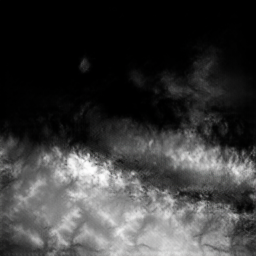
\includegraphics[width=0.25\columnwidth]{02.png} & 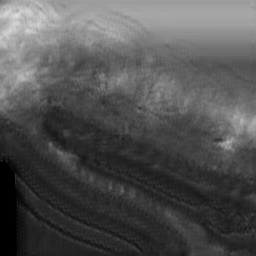
\includegraphics[width=0.25\columnwidth]{03.png} & 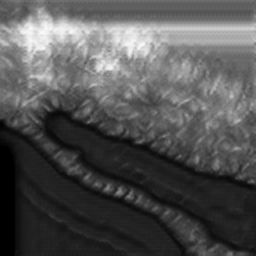
\includegraphics[width=0.25\columnwidth]{04.png} \\
 				
\includegraphics[width=0.25\columnwidth]{10.png} & 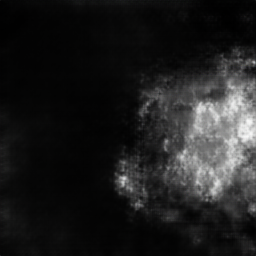
\includegraphics[width=0.25\columnwidth]{11.png} & 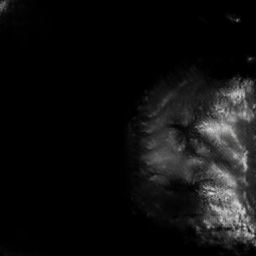
\includegraphics[width=0.25\columnwidth]{12.png} & 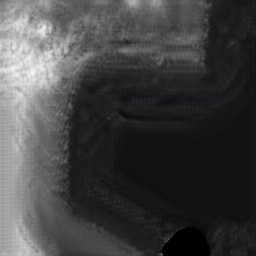
\includegraphics[width=0.25\columnwidth]{13.png} & 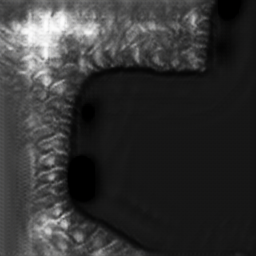
\includegraphics[width=0.25\columnwidth]{14.png} \\
 				
\includegraphics[width=0.25\columnwidth]{20.png} & 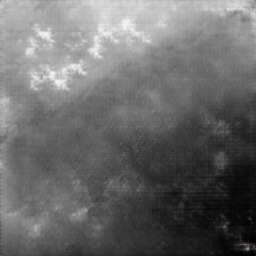
\includegraphics[width=0.25\columnwidth]{21.png} & 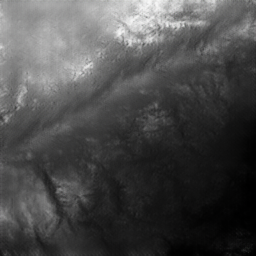
\includegraphics[width=0.25\columnwidth]{22.png} & 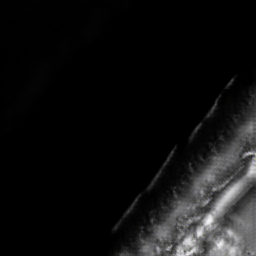
\includegraphics[width=0.25\columnwidth]{23.png} & 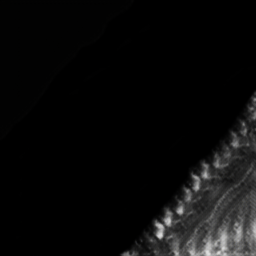
\includegraphics[width=0.25\columnwidth]{24.png} \\
 				
\includegraphics[width=0.25\columnwidth]{30.png} & 
\includegraphics[width=0.25\columnwidth]{31.png} & 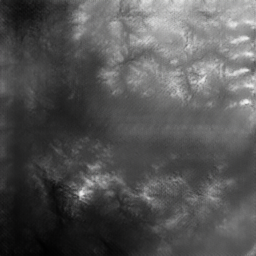
\includegraphics[width=0.25\columnwidth]{32.png} & 
\includegraphics[width=0.25\columnwidth]{33.png} & 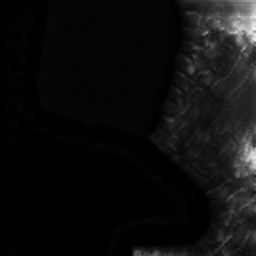
\includegraphics[width=0.25\columnwidth]{34.png} \\
 				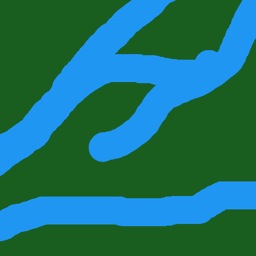
\includegraphics[width=0.25\columnwidth]{40.png} & 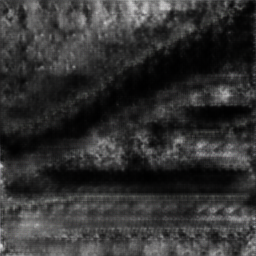
\includegraphics[width=0.25\columnwidth]{41.png} & 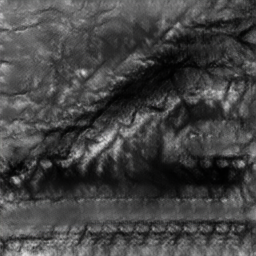
\includegraphics[width=0.25\columnwidth]{42.png} & 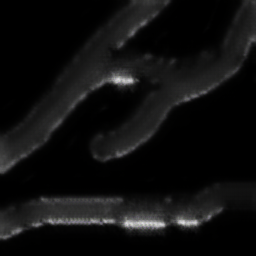
\includegraphics[width=0.25\columnwidth]{43.png} & 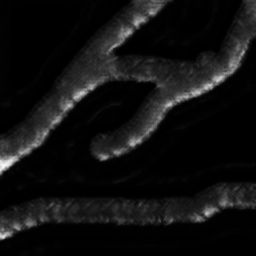
\includegraphics[width=0.25\columnwidth]{44.png} \\
 				
\includegraphics[width=0.25\columnwidth]{50.png} & 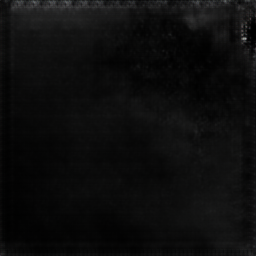
\includegraphics[width=0.25\columnwidth]{51.png} & 
\includegraphics[width=0.25\columnwidth]{52.png} & 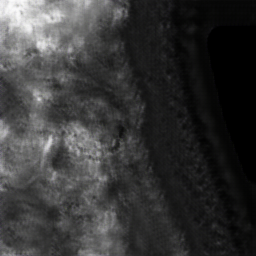
\includegraphics[width=0.25\columnwidth]{53.png} & 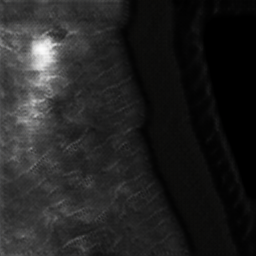
\includegraphics[width=0.25\columnwidth]{54.png} \\
 				
\includegraphics[width=0.25\columnwidth]{60.png} & 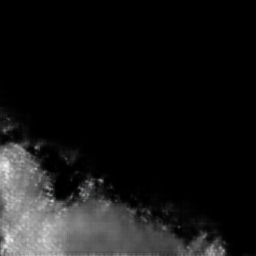
\includegraphics[width=0.25\columnwidth]{61.png} & 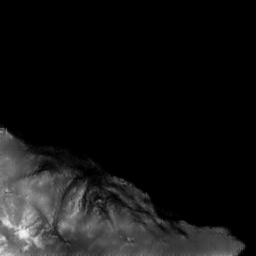
\includegraphics[width=0.25\columnwidth]{62.png} & 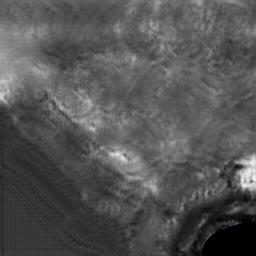
\includegraphics[width=0.25\columnwidth]{63.png} & 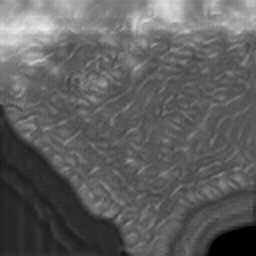
\includegraphics[width=0.25\columnwidth]{64.png} \\
 				
\includegraphics[width=0.25\columnwidth]{70.png} & 
\includegraphics[width=0.25\columnwidth]{71.png} & 
\includegraphics[width=0.25\columnwidth]{72.png} & 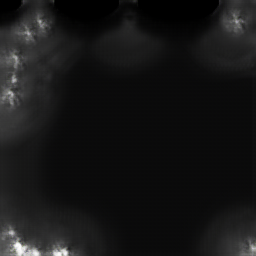
\includegraphics[width=0.25\columnwidth]{73.png} & 
\includegraphics[width=0.25\columnwidth]{74.png} \\
 				
\includegraphics[width=0.25\columnwidth]{80.png} & 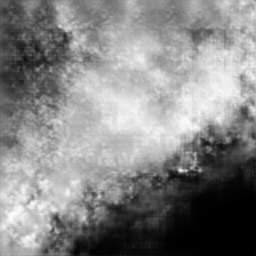
\includegraphics[width=0.25\columnwidth]{81.png} & 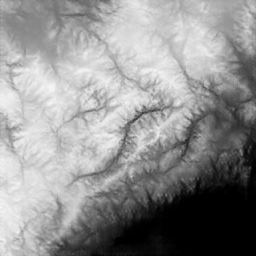
\includegraphics[width=0.25\columnwidth]{82.png} & 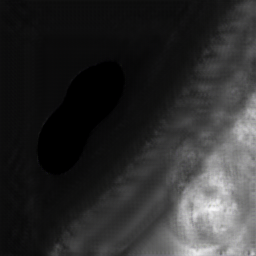
\includegraphics[width=0.25\columnwidth]{83.png} & 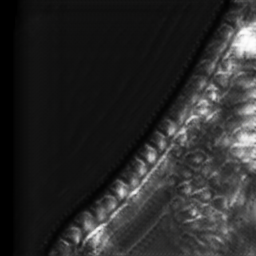
\includegraphics[width=0.25\columnwidth]{84.png} \\
 				
\includegraphics[width=0.25\columnwidth]{90.png} & 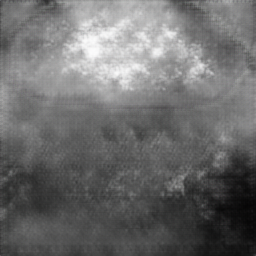
\includegraphics[width=0.25\columnwidth]{91.png} & 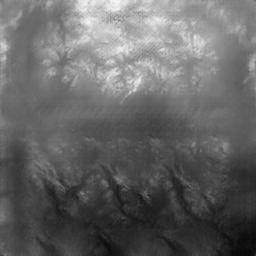
\includegraphics[width=0.25\columnwidth]{92.png} & 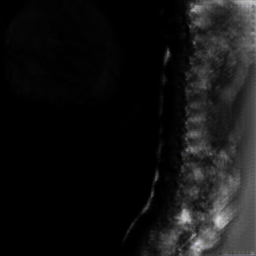
\includegraphics[width=0.25\columnwidth]{93.png} & \includegraphics[width=0.25\columnwidth]{94.png} \\

		\end{tabular}
		
		\caption{Test images and the outputs from our trained models}
	\end{table*}

	\section{Conclusion}
	
	We saw that we can generate good results with generative adversarial networks. It's easy to generate these environments faster and more efficiently than traditional methods.
	
	Using heightmaps as a target allows for the resulting environments to be generalizable. We can import the heightmaps into many popular 3d software applications like Unity, Unreal and Blender.
	
	The training time is computationally intensive, but inference is quick. Once a model is trained, it's easy to generate as many new environments as you want. This has massive improvements over hand crafted environments.
	
	Pix2Pix performs much better than CycleGAN and users prefer its output for this task over CycleGAN for every sample. Pix2Pix offers specificty that CycleGAN can not match.
	
	This is a viable area of research, and there's opportunities to tune these models further to get better results. Training data is the most important part of this project, and spending more time with it will lead to better results. We also show that augmenting the training data is an easy way to expand a dataset, but it can lead to overfitting. There is a middleground between too much and too little for augmentation.
	
	\subsection{Future Work}
	
	Expanding this idea to include texture maps could be an interesting direction to go. Using this same method, it should be possible to translate a given heightmap into a texturemap. This could allow the designer to have control over generated styles like barren desert scenes vs dark horror scenes vs fantastical colorful scenes. Gathering training data of texturemaps would likely be the bottleneck.
	
	Modifying the network to perform real time generation would be an interesting addition. This would give the user a more interactive experience in designing the enviroments. Current latency with this implementation is not fast enough so new network architectures or approaches would be needed.
	
	Tunable paramaters would also be an interesting addition. Giving the user even more control over the results would lead to a better experience. I can imagine parameters like intensity, noise, smoothness could rusult in a lot of usable outcomes.
	
	Expanding the training set with different means. Needing to draw all the usermaps for the training set is time consuming and error/bias prone. Coming up with a programmatic way to create the usermap training set could have a large impact on the quality of the results.

	\bibliographystyle{plain}
	\bibliography{references}
	
	\clearpage
	
	\begin{figure}[h!]
	\caption{Sample usermaps, generated heightmaps, and visualized 3d terrain}	
	\includegraphics[width=2\columnwidth]{viz-1.png} 
	\end{figure}
	
	\begin{figure}[h!]
	\includegraphics[width=2\columnwidth]{viz-2.png} 
	\end{figure}
	
	\begin{figure}[h!]
	\includegraphics[width=2\columnwidth]{viz-3.png} 
	\end{figure}
		
  
\end{document}